% questions.tex —— 1977 年·福建卷·文科 · 题目内容片段（无答案）
% 由 tools/generate_projects.py 依来源总账自 1977/1977_数学真题_福建文_试题.md 生成，勿手改（改源 MD 后重跑）


\gkpart{文科数学（福建卷）}

\begin{gktip}
\textbf{来源说明}：本题面依据固定源 PDF《1977 年普通高等学校招生考试（福建卷）文科数学》单页扫描逐题转录。源文件为 A3 单页题面，正式题为第 1—6 题。第 3(2)、第 4、第 5 和第 6 题存在源面信息不足、题意歧义或参数异常，均按源页保留并在答案要点、解析正文和问题总账中标明，未据模型记忆补写。
\end{gktip}

\Needspace{0.4\textheight}
\begin{question}
\gkti{1}

\Needspace{5\baselineskip}
（1） 计算：

\nopagebreak[4]
\[
5-3\times\left[\left(-3\frac38\right)^{-\frac13}+1031\times\left(0.25-2^{-2}\right)\right]\div9^0
\]

（2） 求 $\cos(-840^\circ)$ 的值。

\Needspace{5\baselineskip}
（3） 化简：

\nopagebreak[4]
\[
\sqrt{(2x-3)^2}
\]

（4） 如图，在 $\triangle ABC$ 中，$MN\parallel BC$，$MN=1\ \mathrm{cm}$，$BC=3\ \mathrm{cm}$，$BM=AM+2$，求 $AM$ 的长。
\nopagebreak[4]
\begin{center}% 1977 年福建卷文科第 1(4) 题：三角形中的平行截线
\begin{tikzpicture}[scale=0.85]
  \coordinate (A) at (2.4,3.5);
  \coordinate (B) at (0,0);
  \coordinate (C) at (5.1,0);
  \coordinate (M) at ($(A)!0.42!(B)$);
  \coordinate (N) at ($(A)!0.42!(C)$);
  \draw[thick] (A)--(B)--(C)--cycle;
  \draw[thick] (M)--(N);
  \fill (A) circle (1.2pt) node[above] {$A$};
  \fill (B) circle (1.2pt) node[below left] {$B$};
  \fill (C) circle (1.2pt) node[below right] {$C$};
  \fill (M) circle (1.2pt) node[left] {$M$};
  \fill (N) circle (1.2pt) node[right] {$N$};
\end{tikzpicture}
\end{center}
\nopagebreak[4]
（5） 已知 $\lg3=0.4771$，$\lg x=3.4771$，求 $x$。

\Needspace{5\baselineskip}
（6） 求

\nopagebreak[4]
\[
\lim_{x\to1}\frac{x-1}{x^2-3x+2}
\]

（7） 求函数 $y=x^2+2x-4$ 的极小值。

（8） 已知 $\sin\alpha=\dfrac35$，$\dfrac\pi2<\alpha<\pi$，求 $\tan\alpha$ 的值。

\Needspace{5\baselineskip}
（9） 写出等比数列

\nopagebreak[4]
\[
-\frac29,\quad \frac2{27},\quad -\frac2{81},\quad\cdots
\]

的通项公式。

\end{question}
\begin{question}
\gkti{2}

\Needspace{5\baselineskip}
（1） 求函数

\nopagebreak[4]
\[
y=\frac{\lg(2-x)}{\sqrt{x-1}}
\]

的定义域。

\Needspace{5\baselineskip}
（2） 证明：

\nopagebreak[4]
\[
(\sin\alpha-\cos\alpha)^2+\sin2\alpha=1
\]

\Needspace{5\baselineskip}
（3） 解方程：

\nopagebreak[4]
\[
2\sqrt{x-3}+6=x
\]

\Needspace{5\baselineskip}
（4） 解不等式：

\nopagebreak[4]
\[
x^2-x-6<0
\]

\Needspace{5\baselineskip}
（5） 把分母有理化：

\nopagebreak[4]
\[
\sqrt{\frac{\sqrt5+\sqrt2}{\sqrt5-\sqrt2}}
\]

（6） 某中学革命师生自己动手油漆一个直径为 $1.2\ \mathrm m$ 的地球仪，如果每平方米面积需要油漆 $150$ 克，问共需油漆多少克？（答案保留整数。）

\end{question}
\begin{question}
\gkti{3}某农机厂开展“工业学大庆”运动，在十月份生产拖拉机 $1000$ 台。这样，一月至十月的产量恰好完成全年生产任务。工人同志为了加速农业机械化，计划在年底前再生产 $2310$ 台。

（1） 求十一月、十二月份每月增长率；

（2） 原计划年产拖拉机多少台？

\end{question}
\begin{question}
\gkti{4}求抛物线 $y^2=9x$ 和圆 $x^2+y^2=36$ 在第一象限的交点处的切线方程。

\end{question}
\begin{question}
\gkti{5}已知双曲线

\nopagebreak[4]
\[
\frac{x^2}{24\alpha}-\frac{y^2}{16\cot\alpha}=1\quad(\alpha\text{ \text{为锐角}})
\]

和圆 $(x-m)^2+y^2=r^2$ 相切于点 $A(4\sqrt3,4)$，求 $\alpha\text{、}m\text{、}r$ 的值。

\Needspace{0.4\textheight}
\end{question}
\begin{question}
\gkti{6}某大队在农田基本建设的规划中，要测定被障碍物隔开的两点 $A\text{、}P$ 之间的距离。他们土法上马，在障碍物的两侧选取两点 $B$ 和 $C$（如图），测得 $AB=AC=50\ \mathrm m$，$\angle BAC=60^\circ$，$\angle ABP=120^\circ$，$\angle ACP=135^\circ$，求 $A$ 和 $P$ 之间的距离。（答案可用最简根式表示。）
\nopagebreak[4]
\begin{center}% 1977 年福建卷文科第 6 题：障碍物两侧测距示意图
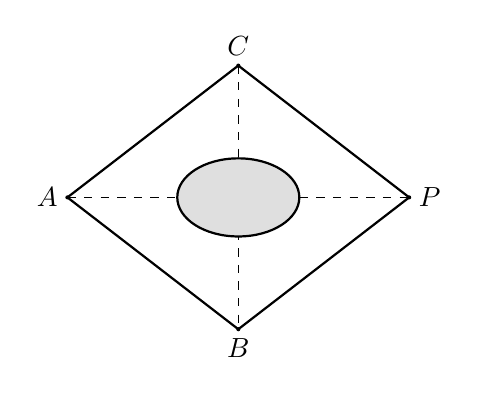
\begin{tikzpicture}[scale=0.62]
  \coordinate (A) at (0,0);
  \coordinate (P) at (7.0,0);
  \coordinate (C) at (3.5,2.7);
  \coordinate (B) at (3.5,-2.7);
  \draw[thick] (A)--(C)--(P)--(B)--cycle;
  \draw[dashed] (A)--(P);
  \draw[dashed] (C)--(B);
  \fill[gray!25] (3.5,0) ellipse (1.25 and 0.8);
  \draw[thick] (3.5,0) ellipse (1.25 and 0.8);
  \fill (A) circle (1.2pt) node[left] {$A$};
  \fill (P) circle (1.2pt) node[right] {$P$};
  \fill (C) circle (1.2pt) node[above] {$C$};
  \fill (B) circle (1.2pt) node[below] {$B$};
\end{tikzpicture}
\end{center}
\nopagebreak[4]

\end{question}